% FractureTAU workshop draft (PAPER-01, D-12 done-definition).
% Self-contained article class so it compiles with `tectonic main.tex` without
% external workshop .sty files. Shell-escape stays OFF (tectonic default).
% NEVER leak any cluster, storage, or user paths here (grep-gated, T-05-22).
\documentclass[11pt]{article}

\usepackage[margin=1in]{geometry}
\usepackage{graphicx}
\usepackage{booktabs}
\usepackage{amsmath}
\usepackage{amssymb}
\usepackage{multirow}
\usepackage{siunitx}
\usepackage[numbers]{natbib}
\usepackage[colorlinks=true,allcolors=blue]{hyperref}

\graphicspath{{figures/}}

\title{Physically-Faithful Fracture Forecasting:\\
A SimVP--TAU Model that Outperforms a Reproduced ConvLSTM Baseline\\
under Autoregressive Rollout}

\author{Juan Ignacio Cantarella \quad Marisol Koslowski\\
Purdue University, West Lafayette, IN, USA\\
\texttt{(SURF 2026 --- workshop draft)}}

\date{\today}

\begin{document}
\maketitle

\begin{abstract}
We study autoregressive (AR) forecasting of spatiotemporal fracture evolution in
simulated microstructures, where a model must roll its own predictions forward
for hundreds of frames. We introduce \textbf{FractureTAU}, a SimVP
encoder/decoder coupled to a Temporal Attention Unit (TAU) translator, trained
in two stages (teacher-forced, then AR fine-tuning with scheduled sampling) with
a Tversky-augmented segmentation loss. Against a \emph{faithfully reproduced}
from-scratch ConvLSTM reference evaluated under an identical AR protocol,
FractureTAU attains a late-rollout (last-20\%) macro $F_1$ of
\textbf{0.8621} (3-seed mean) versus \textbf{0.5767} for the ConvLSTM, a mean
improvement of $+0.285$ that holds on \textbf{16/16} test cases (one-sided
Wilcoxon signed-rank, exact, $n{=}16$: $W{=}136.0$, $p{=}\num{1.526e-5}$).
Beyond the headline $F_1$, we report a battery of physical-fidelity metrics
(boundary localization, crack length and onset, teacher-forced-vs-AR error
accumulation, and probability calibration) showing the improvement reflects more
physically faithful crack forecasts, not a thresholding artifact. We report all
results as mean$\pm$std across three seeds rather than claiming bit-determinism.
\end{abstract}

\section{Introduction}
\label{sec:intro}

Predicting how cracks nucleate and propagate through heterogeneous
microstructures is a long-standing goal in computational materials science.
Surrogate models that forecast the spatiotemporal evolution of a fracture field
could replace expensive physics simulations in design loops, but only if they
remain faithful over long \emph{autoregressive} (AR) rollouts, where the model
consumes its own previous predictions. Teacher-forced metrics, which feed ground
truth at every step, systematically overstate skill; the honest test is
continuous AR rollout, under which errors compound.

We address this setting with \textbf{FractureTAU}, a spatiotemporal predictor
built from a SimVP~\citep{gao2022simvp} encoder/decoder and a Temporal Attention
Unit (TAU)~\citep{tan2023tau} translator. Our contributions are:
\begin{itemize}
  \item \textbf{FractureTAU} (Sec.~\ref{sec:method}): a SimVP+TAU model trained
        with a two-stage teacher-forced$\rightarrow$AR schedule and a
        Tversky-augmented loss tuned for the recall-limited crack-nucleation
        regime.
  \item A \textbf{head-to-head AR win with significance} (Sec.~\ref{sec:results})
        over a faithfully reproduced ConvLSTM reference: $+0.285$ mean macro
        $F_1$, $16/16$ cases, Wilcoxon $p{=}\num{1.526e-5}$.
  \item A \textbf{physical-fidelity analysis} (Sec.~\ref{sec:phys}) integrating
        boundary localization, crack length/onset, TF--AR error accumulation,
        and calibration, so the win is grounded in fracture physics rather than
        a single scalar.
  \item A \textbf{faithful from-scratch baseline reproduction}
        (Sec.~\ref{sec:repro-baseline}) at an honest, verifiable scope, used as a
        credibility anchor for the comparison.
\end{itemize}

\section{Related Work}
\label{sec:related}

\paragraph{Spatiotemporal / video prediction.}
Recurrent convolutional models such as ConvLSTM~\citep{shi2015convlstm},
PredRNN~\citep{wang2017predrnn}, and E3D-LSTM~\citep{wang2019e3dlstm} established
strong baselines for next-frame prediction. More recently, SimVP~\citep{gao2022simvp}
showed that a purely convolutional encoder/decoder with a learned temporal
translator rivals recurrent designs, and TAU~\citep{tan2023tau} introduced an
attention-based translator that decomposes temporal dependencies into intra-frame
(statical) and inter-frame (dynamical) components. FractureTAU adopts the
SimVP+TAU recipe and specializes it for binary fracture-mask forecasting.

\paragraph{ML for fracture.}
Deep models have been used to predict fracture patterns and mechanisms in
crystalline and 2D materials~\citep{hsu2020fracture,lew2021fracture}. A
complementary line of work casts crack evolution as a PDE-surrogate problem:
operator-learning methods such as the Fourier Neural Operator~\citep{li2021fno}
learn solution maps for parametric PDEs, and variational DeepONets have been
specialized to predict crack paths in brittle materials~\citep{goswami2022deeponet}.
Closest to our forecasting task, recent frameworks target rapid forecasting of
crack propagation directly~\citep{yan2024crackforecast}, while benchmarking studies
quantify how well ML surrogates expedite phase-field simulations of brittle
fracture~\citep{hamdi2025phasefield}. These works target different materials,
geometries, governing physics, and outputs than ours, and---crucially---do not
share our continuous autoregressive rollout protocol.

\paragraph{Non-comparability caveat (positioning, not benchmarking).}
We position FractureTAU \emph{conceptually} against the architectures above. We do
\textbf{not} treat their published numbers as an experimental gate: datasets,
grids, physics, and AR evaluation protocols differ across papers, which makes
cross-paper $F_1$ values incomparable. The only quantitative head-to-head in this
paper is against an in-house ConvLSTM reference reproduced and evaluated under an
\emph{identical} AR rollout protocol on the same data
(Sec.~\ref{sec:repro-baseline}).

\section{Method: FractureTAU}
\label{sec:method}

\paragraph{Architecture.}
FractureTAU is a SimVP-style model. A convolutional \emph{encoder} maps each input
frame to a spatial latent; a TAU \emph{translator} models the temporal evolution
of the stacked latents; and a convolutional \emph{decoder} reconstructs the
predicted next-frame fracture field. Spatial dimensions are padded to a multiple
of four inside the encoder to keep the down/up-sampling stack well-defined on the
$321\times161$ grid. The TAU translator combines an intra-frame statical attention
branch with an inter-frame dynamical attention branch, giving the model an
efficient, attention-based alternative to recurrent temporal mixing.

\paragraph{Two-stage training.}
Training proceeds in two stages. \emph{Stage 1} is teacher-forced: the model
predicts the next frame given ground-truth context windows. \emph{Stage 2}
fine-tunes under autoregressive rollout with \emph{scheduled sampling}, gradually
replacing ground-truth feedback with the model's own predictions so that training
matches the AR test-time distribution. An exponential moving average (EMA) of the
weights is maintained for evaluation.

\paragraph{Loss.}
The segmentation objective combines binary cross-entropy, soft Dice, and a
Tversky term (with $\beta = 0.602$) that asymmetrically penalizes false negatives
to counter the recall-limited nucleation regime, together with a growth-mask
upweighting that emphasizes newly fracturing pixels. After training, the decision
threshold is calibrated by grid-searching AR $F_1$ on the validation set.

\paragraph{Autoregressive protocol.}
Both pipelines share a strict AR rollout protocol. Only the fracture channel
(channel~0) is fed back from the model's own prediction; all auxiliary channels
are supplied from ground truth. A \emph{no-healing} monotonicity constraint,
$\text{state} \leftarrow \max(\text{state}, \widehat{\text{pred}}_{\text{bin}})$,
forbids predicted cracks from disappearing. These constraints are identical for
FractureTAU and the ConvLSTM reference, keeping the comparison apples-to-apples.

\section{Experimental Setup}
\label{sec:setup}

\paragraph{Data and protocol.}
We use a fixed simulation dataset on a $321\times161$ grid with 16 held-out test
cases spanning multiple microstructures and loading velocities. Evaluation is a
continuous AR rollout with the no-healing constraint above. Unless noted, we
report \textbf{late-rollout} macro $F_1$, i.e.\ the per-case macro $F_1$ over the
final 20\% of the rollout, where AR drift is most punishing. $F_1$ is computed
with a degenerate-aware definition (empty/empty frames handled explicitly) to
avoid spurious perfect scores.

\paragraph{Seeds and reporting.}
We train FractureTAU with three seeds (42/43/44) and report mean$\pm$std.
Because bf16 AMP and cuDNN are not byte-deterministic, the seed spread is the
honest run-to-run variation; we never claim bit-determinism.

\section{Results}
\label{sec:results}

\subsection{Head-to-head AR win}
\label{sec:headline}

Table~\ref{tab:headline} reports the per-case late-rollout macro $F_1$ for the
3-seed FractureTAU headline model against the frozen from-scratch ConvLSTM
reference (\texttt{base\_regen}). FractureTAU attains an overall macro $F_1$ of
\textbf{0.8621} versus \textbf{0.5767} for the ConvLSTM, a mean improvement of
$+0.285$ (median $+0.2285$) that is positive on \textbf{all 16 cases}. A
one-sided Wilcoxon signed-rank test (TAU $>$ CNN, exact, $n{=}16$, all nonzero)
gives $W{=}136.0$, $p{=}\num{1.526e-5}$, establishing the win as statistically
significant rather than seed luck.

\begin{table}[t]
\centering
\caption{Per-case late-rollout (last-20\%) macro $F_1$: FractureTAU (3-seed
headline) vs.\ frozen from-scratch ConvLSTM (\texttt{base\_regen}). All deltas
positive (16/16). Overall row is the per-case mean. Significance: one-sided
Wilcoxon $W{=}136.0$, $p{=}\num{1.526e-5}$, $n{=}16$.}
\label{tab:headline}
\small
\begin{tabular}{lccc}
\toprule
Case & FractureTAU & ConvLSTM & $\Delta$ \\
\midrule
test\_MS206\_V100            & 0.9506 & 0.0916 & $+0.8590$ \\
test\_MS206\_V1000           & 0.9674 & 0.7044 & $+0.2630$ \\
test\_MS206\_V200            & 0.9483 & 0.2213 & $+0.7270$ \\
test\_MS206\_V400            & 0.9569 & 0.6537 & $+0.3033$ \\
test\_MS210\_V400            & 0.9321 & 0.6564 & $+0.2757$ \\
test\_MS5\_V150ms\_inc       & 0.5971 & 0.3467 & $+0.2504$ \\
test\_MS5\_V400ms            & 0.9305 & 0.7410 & $+0.1896$ \\
test\_PBX1\_V400\_true       & 0.7240 & 0.3575 & $+0.3665$ \\
test\_PBX\_2\_V400           & 0.7841 & 0.6993 & $+0.0848$ \\
test\_emergency\_horizontal  & 0.8589 & 0.7199 & $+0.1391$ \\
test\_horizontal\_layers\_3  & 0.9390 & 0.5864 & $+0.3526$ \\
test\_horizontal\_layers\_4  & 0.9359 & 0.7693 & $+0.1666$ \\
test\_inclusions\_1\_2       & 0.8520 & 0.6454 & $+0.2066$ \\
test\_inclusions\_2\_2       & 0.9344 & 0.7902 & $+0.1442$ \\
test\_inclusions\_3\_2       & 0.8234 & 0.7400 & $+0.0834$ \\
test\_inclusions\_true\_V400 & 0.6584 & 0.5044 & $+0.1540$ \\
\midrule
\textbf{Overall (mean)}      & \textbf{0.8621} & \textbf{0.5767} & $\mathbf{+0.285}$ \\
\bottomrule
\end{tabular}
\end{table}

\subsection{Seed aggregate}
\label{sec:seeds}

Across the three seeds, the per-case late-rollout $F_1$ is stable for the
strongly-fracturing microstructures (e.g.\ test\_MS206\_V200 $0.9483\pm0.0038$,
test\_MS210\_V400 $0.9321\pm0.0019$) and noisier for the hardest nucleation cases
(test\_MS5\_V150ms\_inc $0.5971\pm0.3230$, test\_inclusions\_true\_V400
$0.6584\pm0.1839$). The overall 3-seed macro $F_1$ is $0.8621$. We report these
as mean$\pm$std; the spread is the honest, non-deterministic run-to-run variation.

\subsection{Compact ablation: input channels}
\label{sec:ablation}

Table~\ref{tab:ablation} summarizes the input-channel ablation that motivates the
\texttt{extra=none} (BASE) headline configuration. Adding a stress-derived channel
(von Mises or strain-energy density, SED) \emph{lowered} overall macro $F_1$ in
the breadth runs, so the headline model uses no extra physics channel. The full
five-row leave-one-out ablation and extended significance tables are deferred to
the appendix (Sec.~\ref{sec:appendix}).

\begin{table}[t]
\centering
\caption{Compact input-channel ablation (overall macro $F_1$). Stress-derived
channels degrade overall accuracy; \texttt{extra=none} is the headline choice.}
\label{tab:ablation}
\small
\begin{tabular}{lc}
\toprule
Input configuration & Overall macro $F_1$ \\
\midrule
\texttt{extra=none} (BASE, headline) & \textbf{0.86} \\
$+$ von Mises stress                 & 0.75 \\
$+$ strain-energy density (SED)      & 0.58 \\
\bottomrule
\end{tabular}
\end{table}

\subsection{Faithful baseline reproduction}
\label{sec:repro-baseline}

The credibility of the head-to-head rests on a baseline that is \emph{retrained},
not merely inherited. We reproduced the original ConvLSTM fracture model of
Martinus~\citep{martinus2024thesis} from scratch in its native TensorFlow/Keras
pipeline and evaluated it under the identical AR protocol. We report this reproduction at an \textbf{honest, verifiable scope of
4 BASE / 2 SED} configurations: the corrupt MS206 SED reference exports were
excluded rather than silently included. The frozen reproduction
(\texttt{base\_regen}) is the reference used throughout Sec.~\ref{sec:headline}.

\paragraph{Provenance.}
For traceability we record the SHA-256 of each trained checkpoint. The three
headline FractureTAU seeds have \texttt{best.pt} hashes \texttt{0f55814f02ae}
(s42), \texttt{6a09694abf51} (s43), and \texttt{f97f429e8d9f} (s44); the ConvLSTM
reference is the frozen \texttt{base\_regen} run. Every number in this section
traces to the committed per-frame metric CSVs from these runs.

\section{Physical-Fidelity Analysis}
\label{sec:phys}

A single $F_1$ scalar can hide whether a model gets the \emph{physics} right. We
therefore evaluate FractureTAU's AR predictions against ground truth along four
complementary physical axes, plus an overall stability view.

\paragraph{Boundary localization (HD95 + boundary-$F_1$).}
On the binarized (no-healing) AR prediction we measure crack-front localization
with the 95th-percentile Hausdorff distance (HD95)~\citep{huttenlocher1993hausdorff}
and the boundary-$F_1$ (BF) score within a 2-pixel tolerance~\citep{csurka2013bfscore}.
Averaged over the 16 cases, FractureTAU attains a macro HD95 of \textbf{39.585
px} and a macro boundary-$F_1$ of \textbf{0.6258}. Localization is excellent on
the strongly-fracturing cases (e.g.\ test\_MS206\_V1000: HD95 $2.56$ px,
BF $0.966$) and degrades on diffuse PBX cases, consistent with the $F_1$ pattern.

\paragraph{Crack length and onset.}
Figure~\ref{fig:length} compares the predicted and ground-truth crack length
(skeleton-pixel count per frame; pixel pitch left at 1.0) and the time-to-onset
(first frame with any predicted crack) for the representative median-$F_1$ case.
FractureTAU tracks the onset timing and growth trend, typically slightly
under-predicting final crack length --- a conservative bias rather than runaway
over-growth.

\begin{figure}[t]
\centering
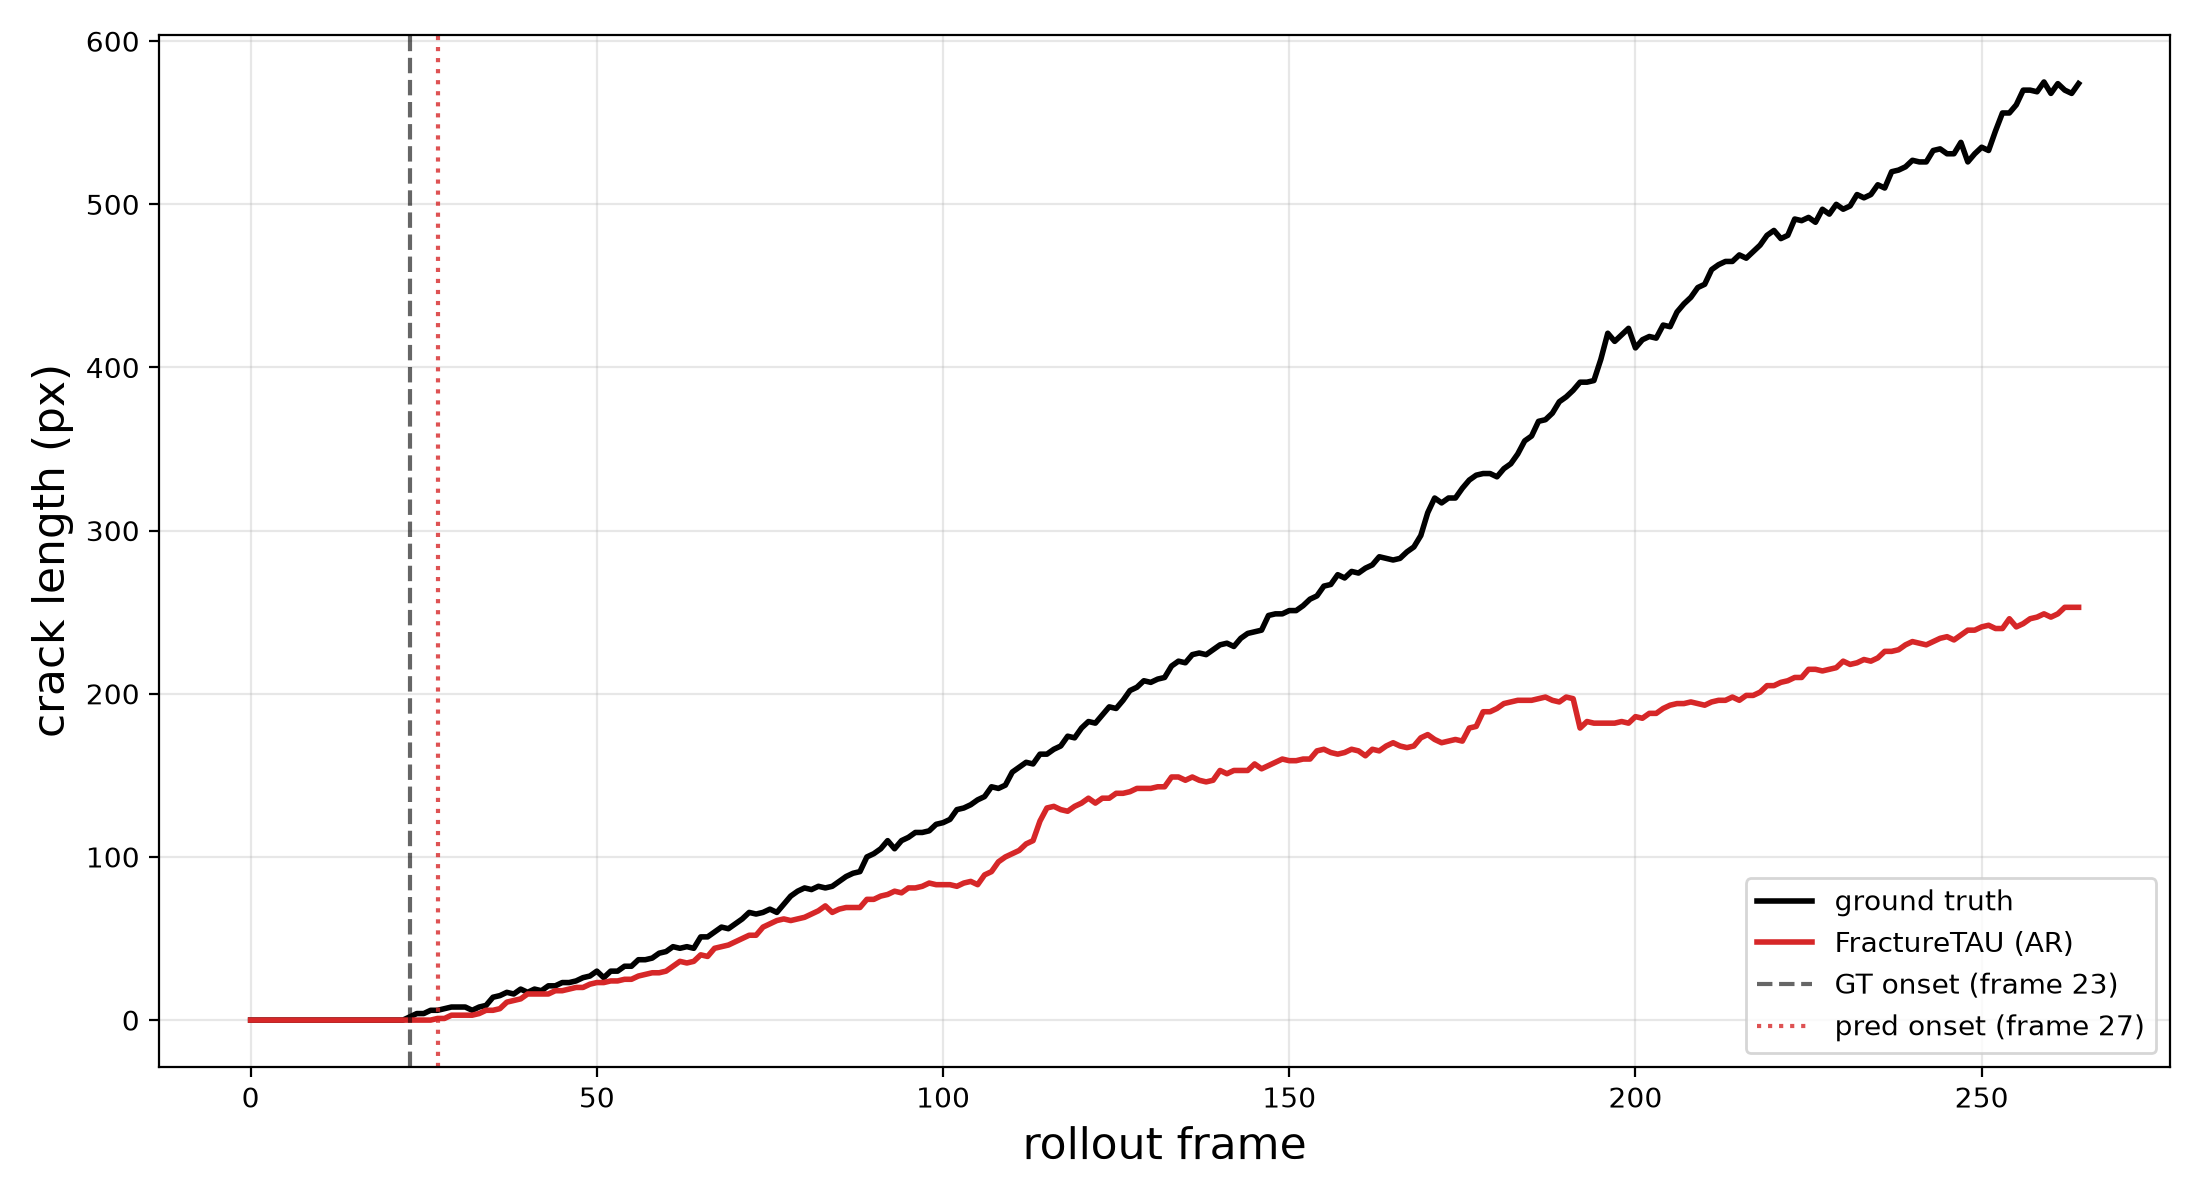
\includegraphics[width=0.72\linewidth]{length_test_emergency_horizontal.png}
\caption{Crack length over time and onset (representative case
test\_emergency\_horizontal): ground truth vs.\ FractureTAU AR prediction. The
model captures onset timing and growth trend, with a mild conservative
under-prediction of final length.}
\label{fig:length}
\end{figure}

\paragraph{Error accumulation: teacher-forced vs.\ autoregressive.}
Figure~\ref{fig:horizon} shows the per-frame $F_1$ gap between the teacher-forced
(TF) pass and the AR rollout over the horizon. The gap quantifies AR drift: it is
small for cleanly-fracturing cases (e.g.\ test\_MS206\_V1000 mean gap $+0.05$) and
larger for hard nucleation/diffuse cases. The TF pass is inference-only and
freeze-legal; both curves use the degenerate-aware $F_1$.

\begin{figure}[t]
\centering
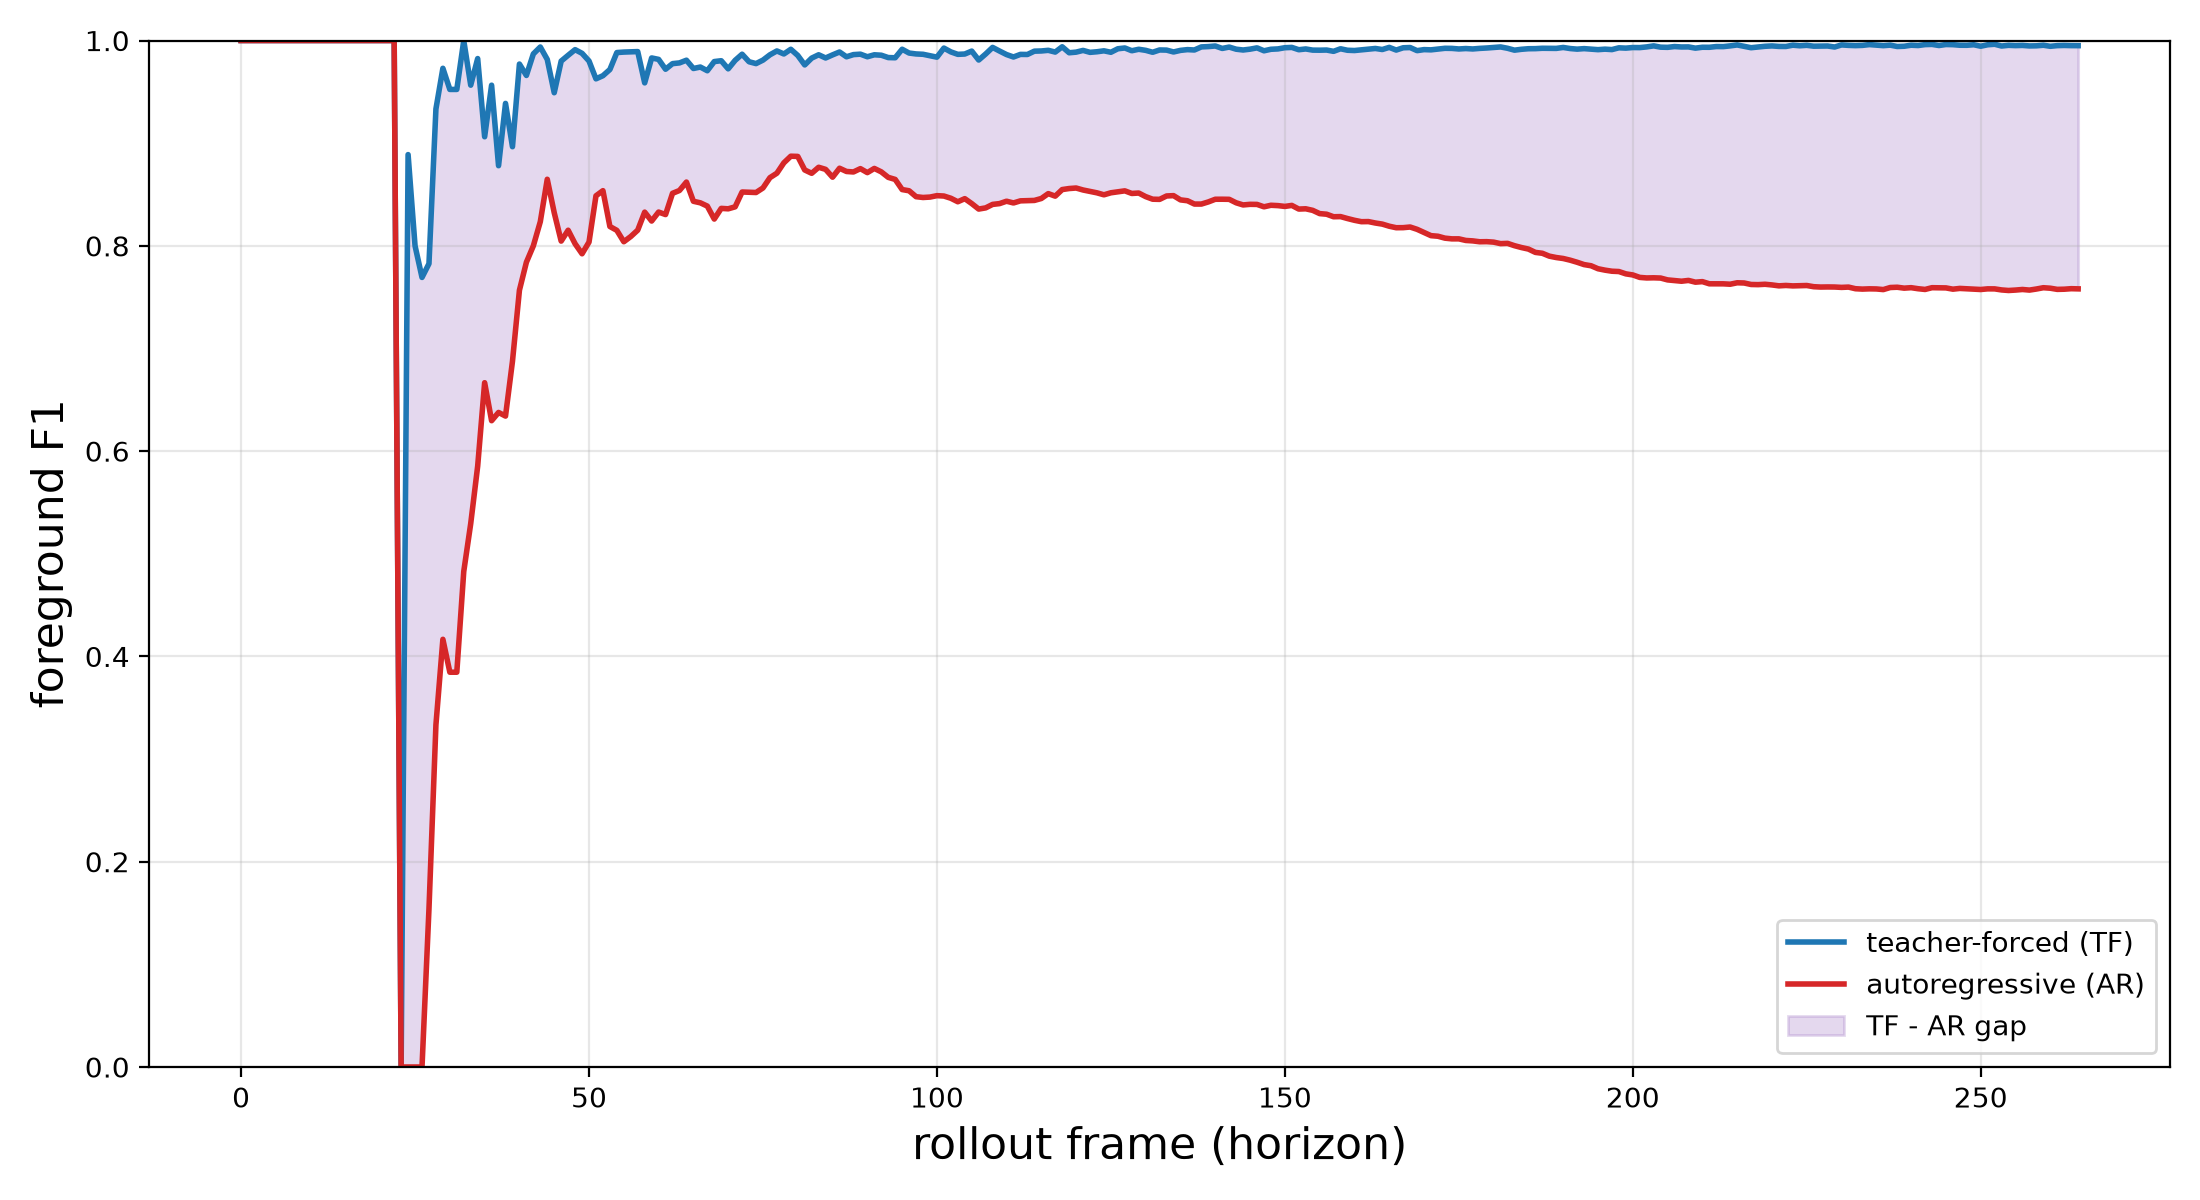
\includegraphics[width=0.72\linewidth]{f1_horizon_test_emergency_horizontal.png}
\caption{Teacher-forced vs.\ autoregressive per-frame $F_1$ over the rollout
horizon (test\_emergency\_horizontal). The TF--AR gap grows with horizon,
quantifying autoregressive error accumulation.}
\label{fig:horizon}
\end{figure}

\paragraph{Rollout stability.}
Figure~\ref{fig:stability} aggregates per-case foreground-$F_1$ curves onto a
common normalized rollout fraction $[0,1]$, showing the median and inter-quartile
band across cases. FractureTAU maintains a high median foreground-$F_1$ across the
full rollout rather than collapsing late, which is the failure mode AR fine-tuning
is designed to prevent.

\begin{figure}[t]
\centering
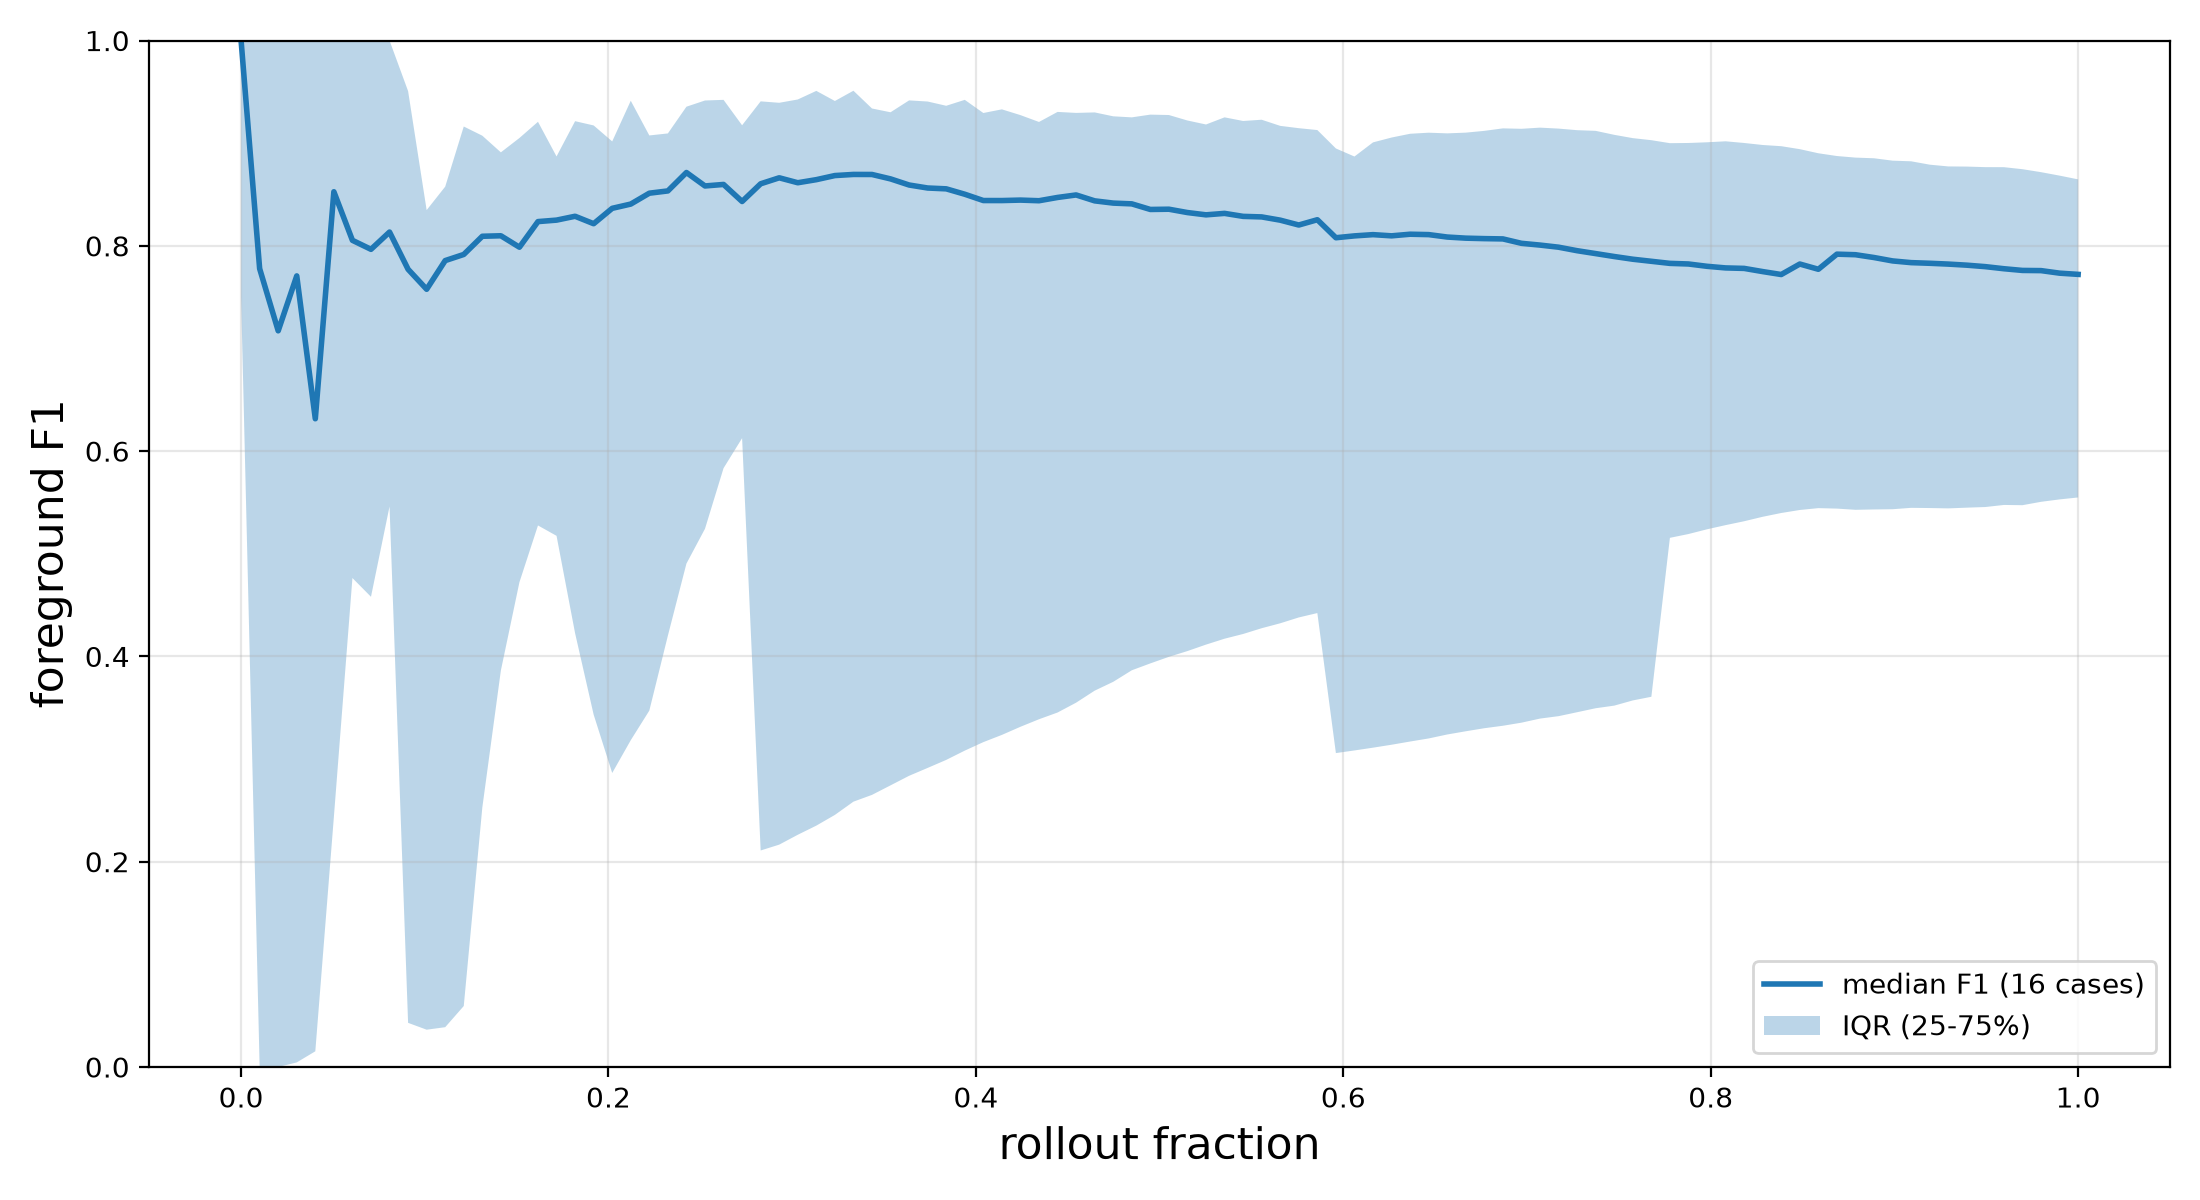
\includegraphics[width=0.72\linewidth]{stability.png}
\caption{Rollout-stability band: per-case foreground-$F_1$ resampled to a common
normalized rollout fraction; line is the median, band is the 25--75\% IQR across
the 16 cases.}
\label{fig:stability}
\end{figure}

\paragraph{Calibration.}
We assess the reliability of the raw predicted probabilities (binned by predicted
probability, never by a binarized mask) and report the Expected Calibration Error
(ECE)~\citep{guo2017calibration}. The aggregate ECE over the 16 cases is
\textbf{0.0435}; the reliability diagram is in the appendix
(Fig.~\ref{fig:reliability}).

\paragraph{Qualitative panels (TODO).}
Spatial false-positive/false-negative overlay panels were not generated for this
draft; we flag them as a TODO rather than fabricate a figure.

\section{Reproducibility}
\label{sec:repro}

All experiments run on a university HPC cluster (Slurm, A100 GPUs) from a
pinned environment (\texttt{uv.lock}) with a documented train/validation split and
seed 42 as the base seed. Because bf16 AMP and cuDNN are not byte-deterministic,
we report results as \textbf{mean$\pm$std over three seeds} rather than claiming
bit-determinism. For compute accounting, FractureTAU has \textbf{10{,}323{,}201}
parameters and \textbf{$\num{2.310e11}$ FLOPs} per forward pass (FLOPs $= 2\times$
MACs), and the headline model trains in \textbf{3.826 A100-hours}. The frozen
ConvLSTM reference is profiled separately in its own TensorFlow environment, since
cross-framework FLOP counters are not directly comparable.

\section{Conclusion}
\label{sec:conclusion}

We presented FractureTAU, a SimVP+TAU spatiotemporal model for autoregressive
fracture forecasting that significantly outperforms a faithfully reproduced
from-scratch ConvLSTM baseline under an identical AR rollout protocol
($0.8621$ vs.\ $0.5767$ late-rollout macro $F_1$; $16/16$ cases;
Wilcoxon $p{=}\num{1.526e-5}$). A physical-fidelity analysis --- boundary
localization, crack length/onset, TF--AR error accumulation, calibration, and
rollout stability --- shows the improvement is physically grounded. Limitations
include the deferred qualitative FP/FN panels and the workshop-scope baseline
reproduction (4 BASE / 2 SED). Future work includes displacement-field
prediction, broader microstructure coverage, and a fuller SOTA positioning study.

\section*{Appendix}
\label{sec:appendix}

\paragraph{Calibration reliability diagram.}
Figure~\ref{fig:reliability} shows the aggregate reliability diagram over all 16
cases (aggregate ECE $0.0435$).

\begin{figure}[tb]
\centering
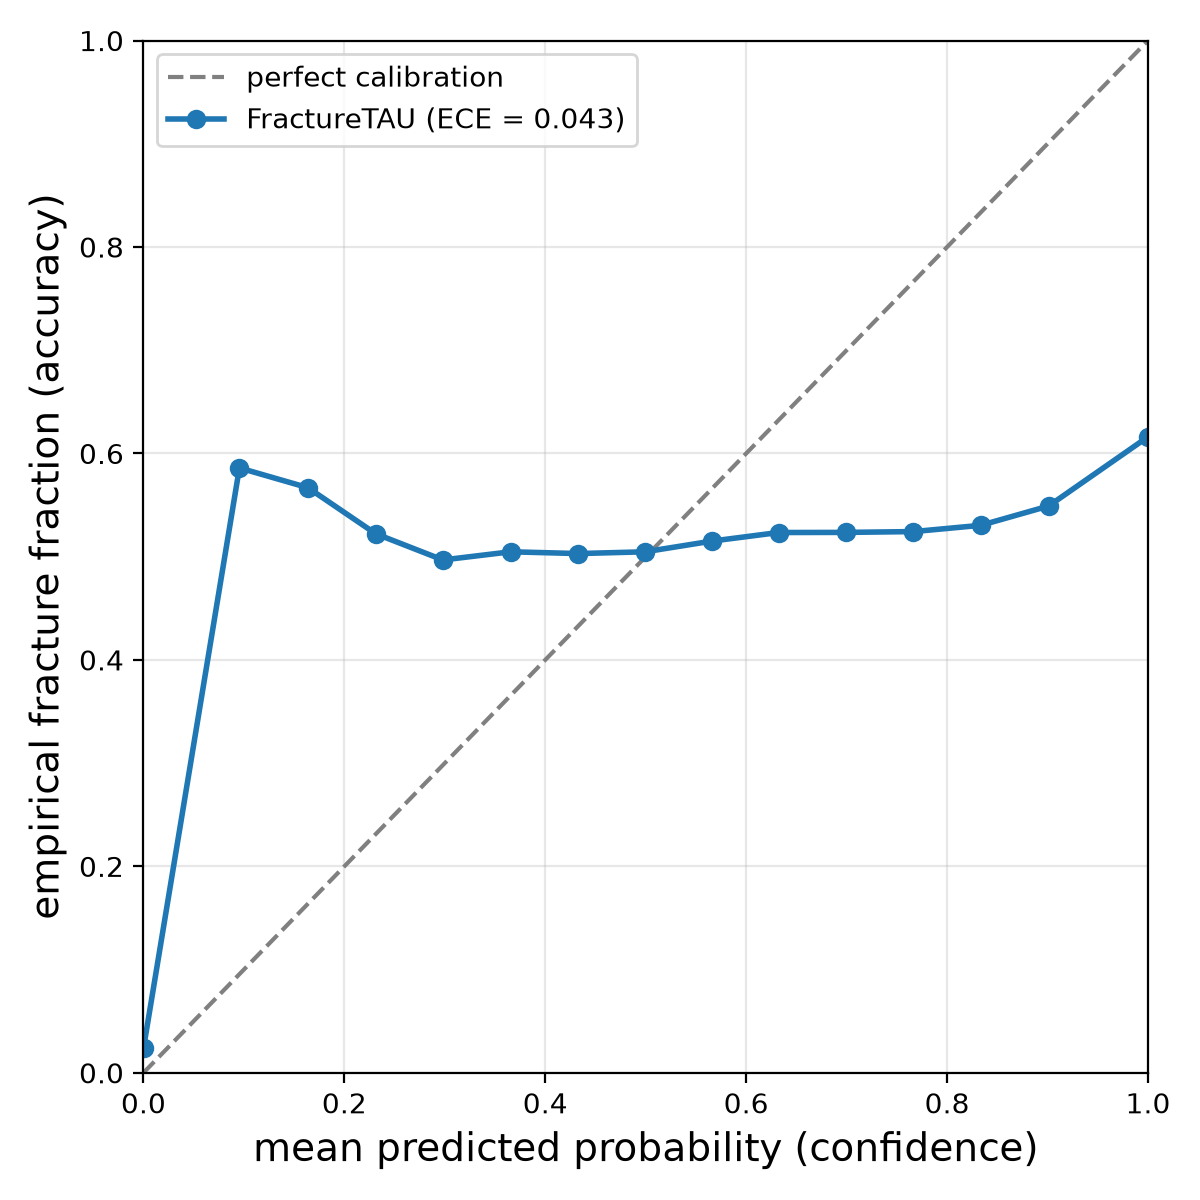
\includegraphics[width=0.6\linewidth]{reliability.png}
\caption{Aggregate reliability diagram over the 16 test cases (ECE $0.0435$),
binned by predicted probability.}
\label{fig:reliability}
\end{figure}

\paragraph{Extended tables.}
The full five-row leave-one-out input ablation and the extended per-seed
significance tables are maintained alongside the measured artifacts and will be
folded into a longer version of this paper.

\section*{Acknowledgments}
This work was carried out under the Summer Undergraduate Research Fellowship
(SURF) program at Purdue University. We thank our mentors Kyle Jung and Joshua
Block for their guidance throughout the project, and we gratefully acknowledge
the foundational ConvLSTM fracture-prediction work of Kathleen
Martinus~\citep{martinus2024thesis}, whose model is reproduced as the reference
baseline in this study.

\clearpage
\bibliographystyle{plainnat}
\bibliography{refs}

\end{document}
